\subsection{Malware Detection}
There are multiple ways to adopt malware detection strategies through Wazuh.
  \begin{itemize}
    \item Rootkits behavior detection
    \item CDB lists and threat intelligence
    \item VirusTotal integration
    \item File integrity monitoring and YARA
    \item ClamAV logs collection
    \item Windows Defender logs collection
    \item Custom rules to detect malware IOCs
    \item Osquery
  \end{itemize}

Among these, we explore CDB lists, VirusTotal integration, YARA scanning and Windows Defender logs collection.

\subsubsection{CDB Lists and Threat Intelligence}

\paragraph{How it works}
Wazuh utilizes CDB lists to cross-reference field values like IP addresses, file hashes, and others, obtained from decoding security events, facilitating the identification and tracking of malware. This functionality extends to leveraging CDB lists alongside the File Integrity Monitoring (FIM) module for enhanced malware detection. The operational framework is detailed as follows:

\begin{enumerate}
    \item \textbf{File Integrity Monitoring:} The FIM module conducts surveillance over designated directories on endpoints, aiming to spot any occurrences such as the inception or alteration of files. It meticulously records the checksums alongside other relevant attributes of the files it monitors.
    
    \item \textbf{Alert Generation:} Upon the creation of an alert by the FIM module, Wazuh's analytical engine proceeds to juxtapose the attributes of the file in question, such as its hash, against the keys housed within a specifically chosen CDB list.
    
    \item \textbf{Alert Management:} Should there be a discovery of a match by the analysis engine, it either triggers or suppresses an alert contingent upon the configuration settings established by the user.
\end{enumerate}

This process underscores Wazuh's capability to not only monitor and record file integrity but also to utilize those findings in conjunction with CDB lists for robust malware detection and response strategies.

\paragraph{Configuration}
\subparagraph{Wazuh server}
\begin{enumerate}
    \item Create a CDB list \texttt{malware-hashes} of known malware hashes and save it to the\\ \texttt{/var/ossec/etc/lists} directory on the Wazuh server.
    \begin{minted}{bash}
vi /var/ossec/etc/lists/malware-hashes
    \end{minted}
    \item Add the known malware hashes to the file as \texttt{key:value} pairs. In this case, you can use the known MD5 hashes of the Mirai and Xbash malware as shown below.
    \begin{minted}{text}
e0ec2cd43f71c80d42cd7b0f17802c73:mirai
55142f1d393c5ba7405239f232a6c059:Xbash
    \end{minted}
    \begin{figure}[H]
        \centering
        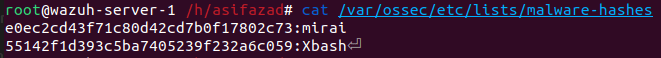
\includegraphics[width=\textwidth]{images/malware-detection/cdb/1.png}
        \caption{List of Malware Hashes (Terminal)}
        \label{fig:malware-hash-1}
    \end{figure}
    Alternatively, these configurations can also be updated from the Wazuh dashboard, like the following:
    \begin{figure}[H]
        \centering
        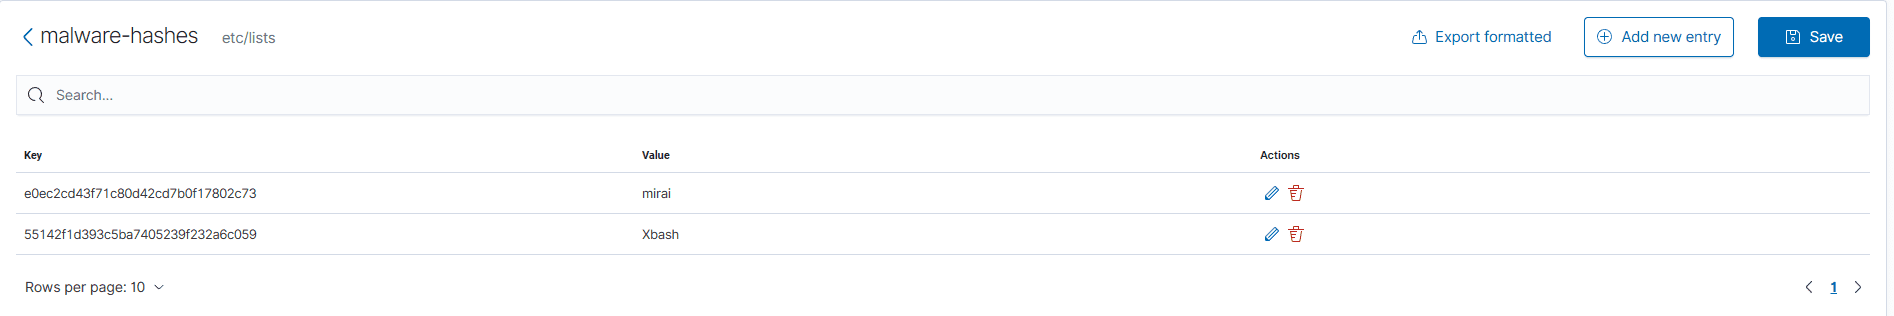
\includegraphics[width=\textwidth]{images/malware-detection/cdb/2.png}
        \caption{List of Malware Hashes (Dashboard)}
        \label{fig:malware-hash}
    \end{figure}
    
    \item Add a reference to the CDB list in the Wazuh manager configuration file \texttt{/var/ossec/etc/ossec.conf}. This can be done by specifying the path to the list within the \texttt{<ruleset>} block:
    \begin{figure}[H]
        \centering
        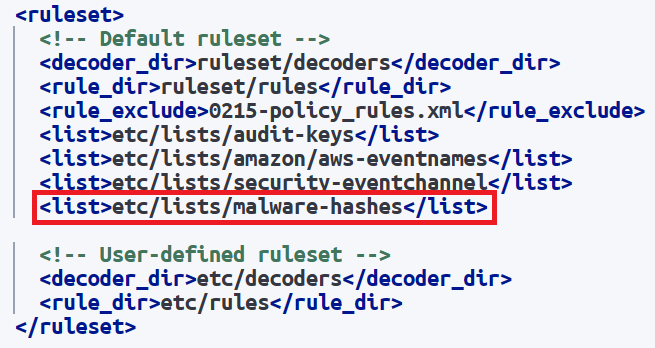
\includegraphics[width=0.65\textwidth]{images/malware-detection/cdb/3.png}
        \caption{Add Malware List to Ruleset}
        \label{fig:malware-list-ruleset}
    \end{figure}
    
    \item Create a custom rule in the \texttt{/var/ossec/etc/rules/local\_rules.xml} file on the Wazuh server. The rule generates alerts when the Wazuh analysis engine matches the MD5 hash of a new or modified file to a hash in the CDB list. Rules 554 and 550 must previously match indicating a recently created or modified file.
    \begin{figure}[H]
        \centering
        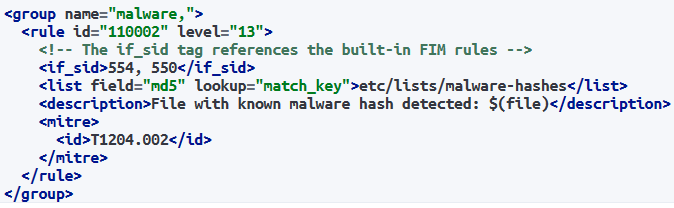
\includegraphics[width=0.75\textwidth]{images/malware-detection/cdb/4.png}
        \caption{Custom Rule added to Server}
        \label{fig:cdb-custom-rule}
    \end{figure}
    \item Restart the Wazuh manager to apply changes.
    \begin{minted}{bash}
systemctl restart wazuh-manager
    \end{minted}
\end{enumerate}

\subparagraph{Linux endpoint}
\label{fim-source}
\begin{enumerate}
    \item Configure directory monitoring by adding the \texttt{\textlangle directories\textrangle} block specifying the folders that need to be monitored in the agent configuration file or using the centralized configuration option. We will monitor the \texttt{/fim} directory here.
    \begin{figure}[H]
        \centering
        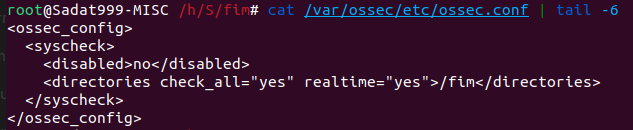
\includegraphics[width=\textwidth]{images/malware-detection/cdb/5.png}
        \caption{Adding a Monitored Directory}
        \label{fig:monitored-dir}
    \end{figure}

    \item Restart the Wazuh agent to apply the changes:
    \begin{minted}{bash}
systemctl restart wazuh-agent
    \end{minted}
\end{enumerate}

\paragraph{Simulation}
To test that everything works correctly, we need to download the Mirai and Xbash malware samples to the directory the FIM module is monitoring.
\begin{enumerate}
    \item We need to download the malware samples.
    \begin{minted}{bash}
sudo curl https://wazuh-demo.s3-us-west-1.amazonaws.com/mirai --output /fim/mirai
sudo curl https://wazuh-demo.s3-us-west-1.amazonaws.com/xbash --output /fim/Xbash
    \end{minted}

    \begin{figure}[H]
        \centering
        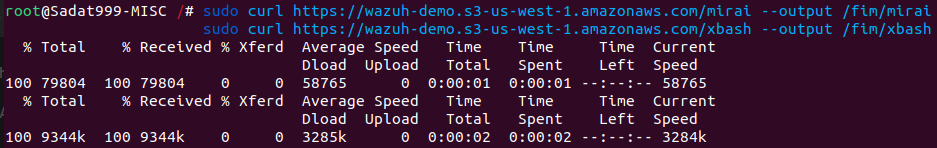
\includegraphics[width=\textwidth]{images/malware-detection/cdb/7.png}
        \caption{Manually Downloading the Malwares}
        \label{fig:malware-download}
    \end{figure}
\end{enumerate}

\paragraph{Dashboard Update}
\label{navigate-sec}
The alerts can be seen on the Wazuh dashboard. To do this, navigate to the following:
    \begin{figure}[H]
        \centering
        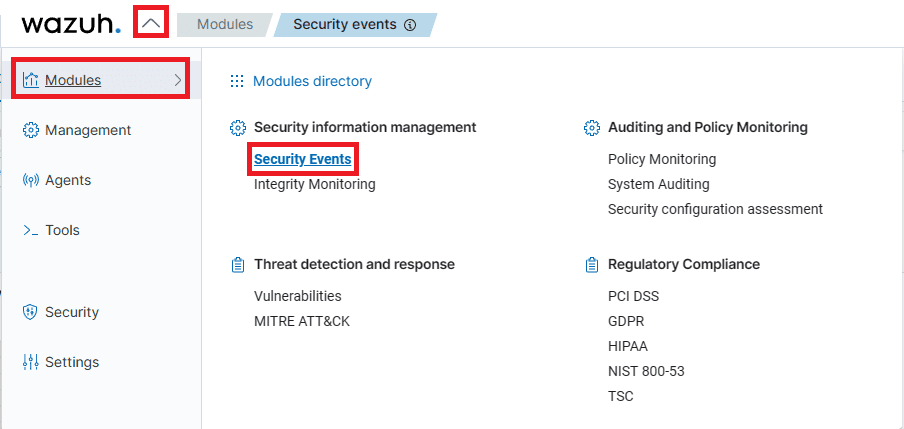
\includegraphics[width=\textwidth]{images/malware-detection/cdb/8.png}
        \caption{Navigation to Security Events}
        \label{fig:navigate-security}
    \end{figure}
As per our defined rules, two level 13 alerts should have been generated, for which the number of level 12 or above alerts is now 15, previously this was 13.
    \begin{figure}[H]
        \centering
        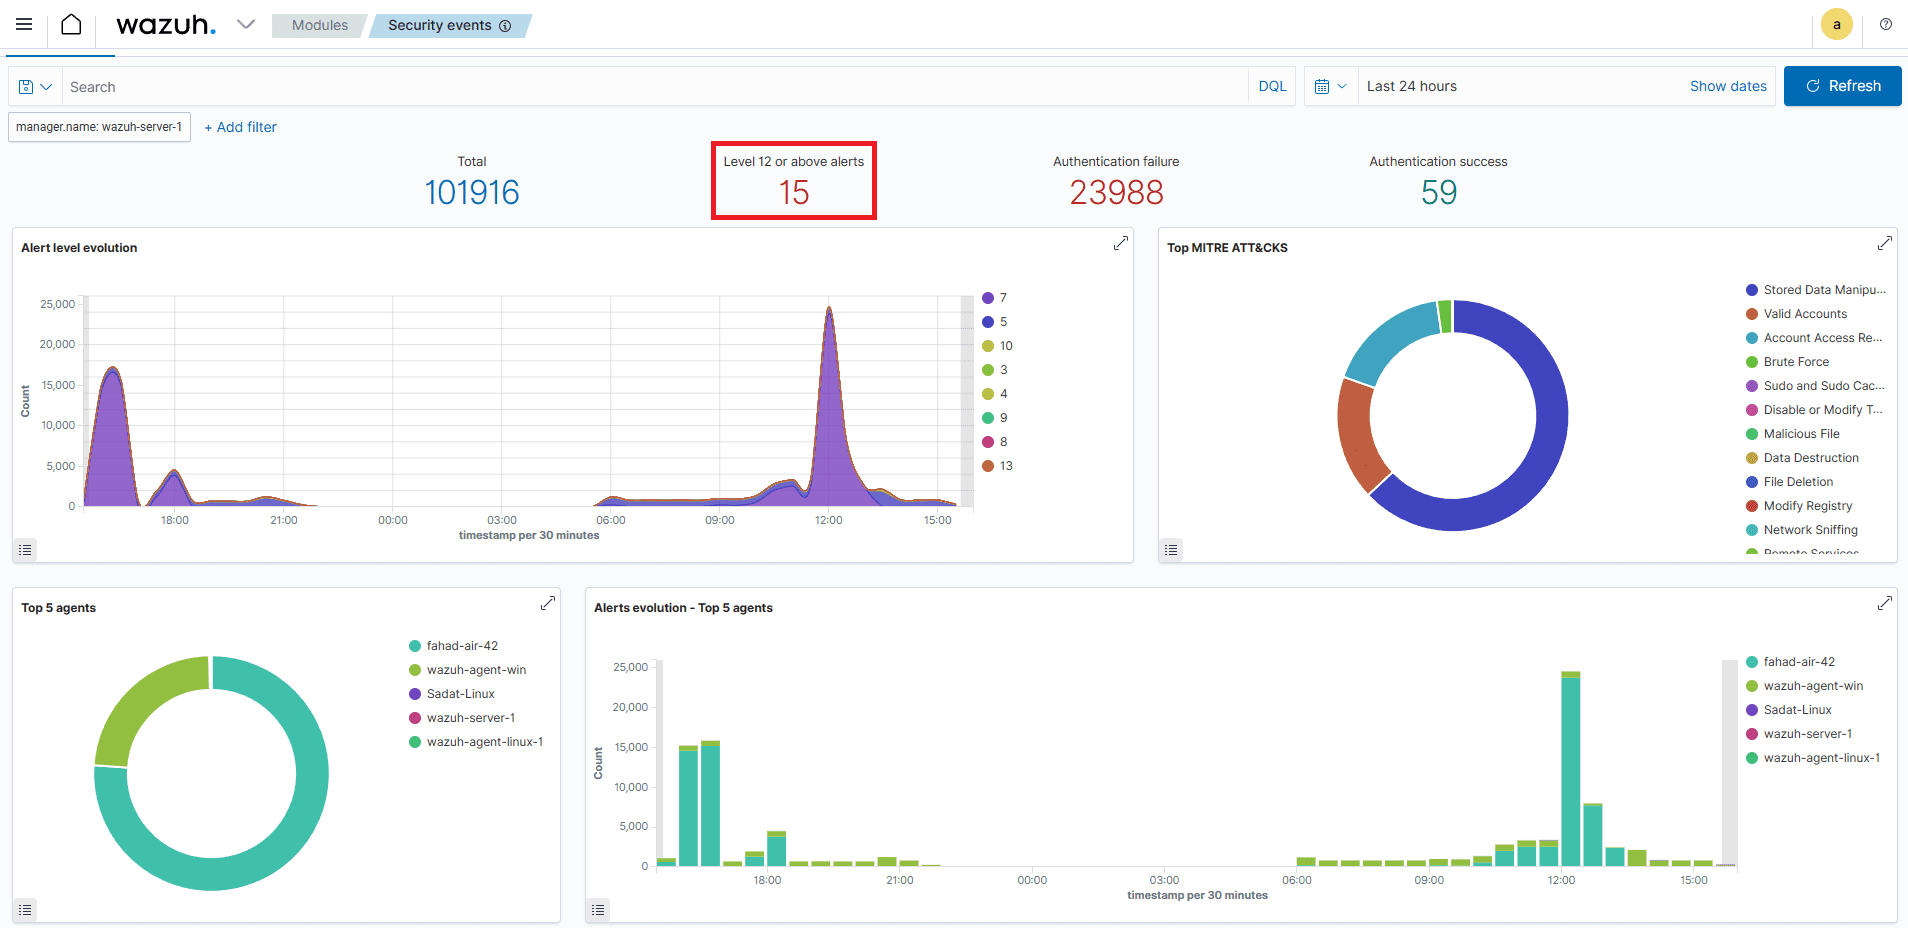
\includegraphics[width=\textwidth]{images/malware-detection/cdb/10.png}
        \caption{Dashboard after Malware Download}
        \label{fig:cdb-post-malware-download}
    \end{figure}
At the bottom, we can see two new alerts have been generated at the latest time because of the two malwares downloaded. We can see further details for them as well upon clicking.
    \begin{figure}[H]
        \centering
        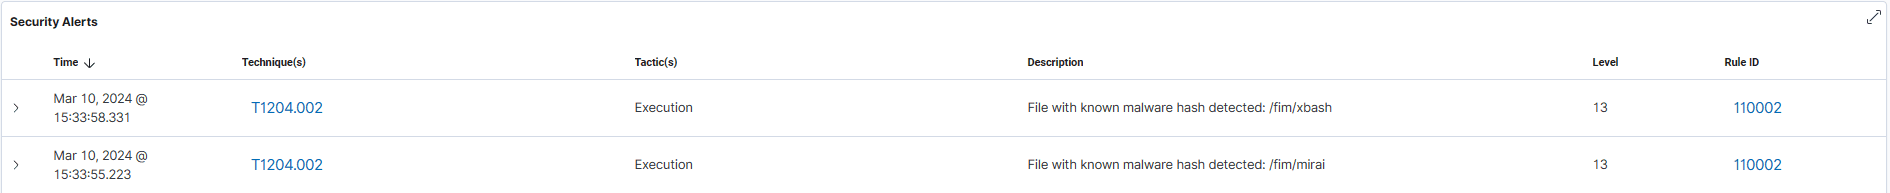
\includegraphics[width=\textwidth]{images/malware-detection/cdb/9.png}
        \caption{Alerts Generated by CDB Matching}
        \label{fig:cdb-alerts}
    \end{figure}

\subsubsection{File Integrity Monitoring and YARA Scanning}
\paragraph{How it works}
This methodology employed for malware detection unfolds through several phases as follows:

\begin{enumerate}
    \item The File Integrity Monitoring (FIM) feature of Wazuh scrutinizes directories on endpoints to identify any alterations, including the creation or modification of files.
    
    \item Upon identifying a modification in any monitored directory or file, FIM initiates a YARA scan as part of its active response mechanism. This is executed through the \texttt{yara.sh} script, which subsequently examines the implicated file against its YARA rules to ascertain if it contains malware.
    
    \item Should the YARA rules find a match for the file, the ensuing scan data is sent to the Wazuh manager for decoding, analysis, and generation of alerts. It's important to note that these scan outcomes are not immediately interpretable and require the integration of specific decoders into your Wazuh server.
\end{enumerate}

The diagram below illustrates the flow of events between the different components.
\begin{figure}[H]
    \centering
    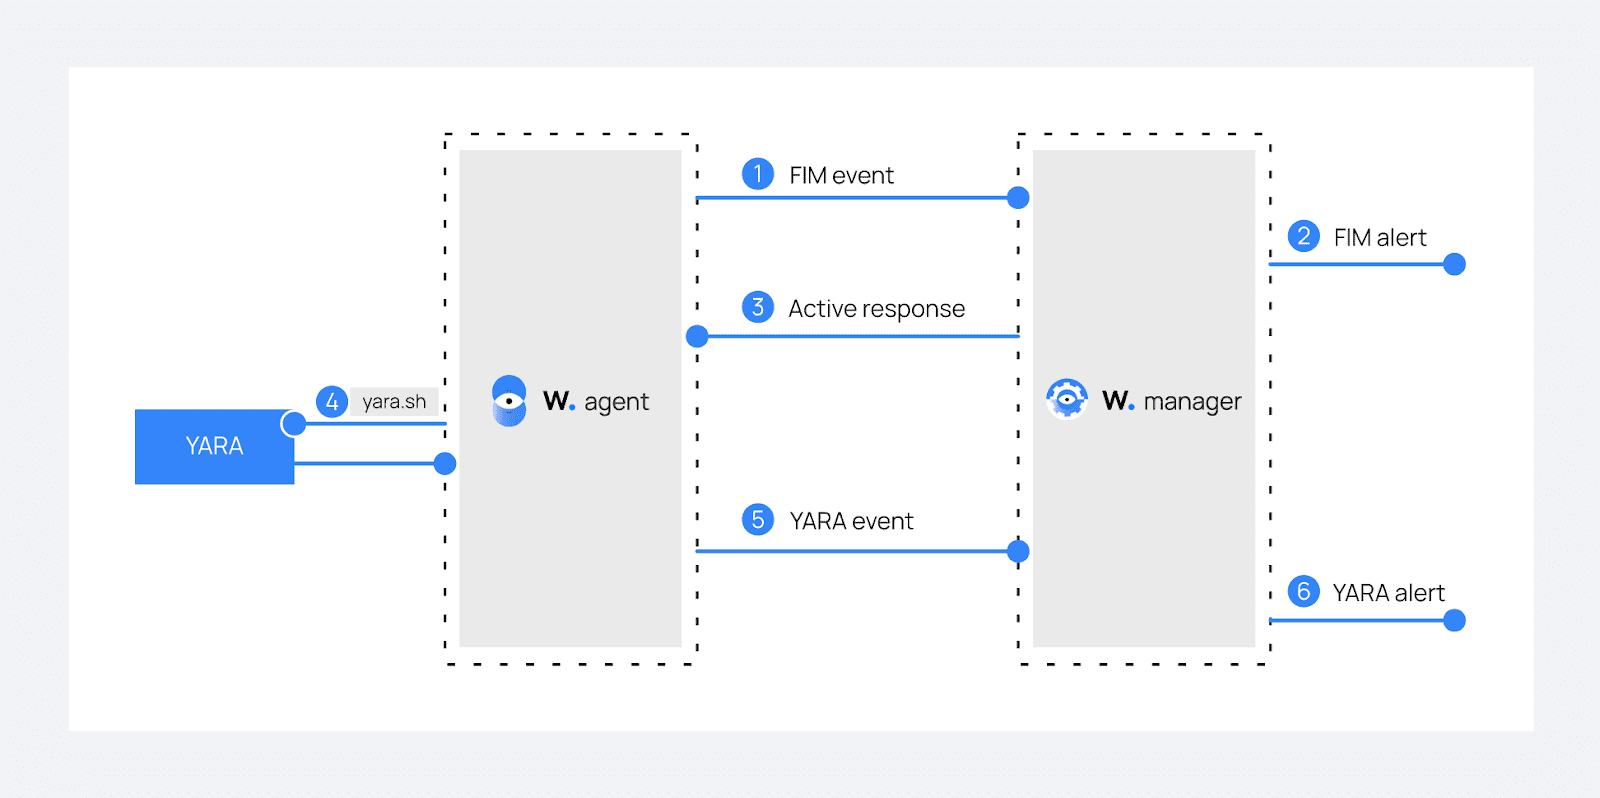
\includegraphics[width=\textwidth]{images/malware-detection/yara/flow.png}
    \caption{Workflow of Malware Detection through YARA scanning}
    \label{fig:yara-flow}
\end{figure}

This YARA scanning procedure, integrated into the active response system, focuses its analysis on either newly created or recently altered files within the monitored directories, thereby ensuring efficient utilization of resources across the endpoints.

\paragraph{Configuration}

\subparagraph{Linux endpoint}
\begin{enumerate}
    \item Download, compile, and install YARA:
    \begin{minted}{bash}
sudo apt update
sudo apt install -y make gcc autoconf libtool libssl-dev pkg-config
sudo curl -LO https://github.com/VirusTotal/yara/archive/v4.2.3.tar.gz
sudo tar -xvzf v4.2.3.tar.gz -C /usr/local/bin/ && rm -f v4.2.3.tar.gz
cd /usr/local/bin/yara-4.2.3/
sudo ./bootstrap.sh && sudo ./configure && sudo make && sudo make install && sudo make check
    \end{minted}

    \item Test that YARA is running properly.
\begin{figure}[H]
    \centering
    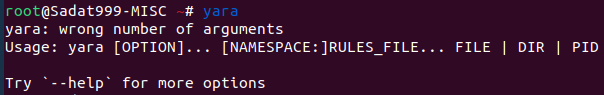
\includegraphics[width=0.8\textwidth]{images/malware-detection/yara/1.png}
    \caption{Checking YARA Installation}
    \label{fig:yara-check}
\end{figure}
    If it asks for right number of arguments as shown in the image above, then the installation has worked correctly. However, an error might occur saying that shared object file can't be opened. This means that the loader doesn’t find the \texttt{libyara} library usually located in \texttt{/usr/local/lib}. The path \texttt{/usr/local/lib} has to be added to the \texttt{/etc/ld.so.conf} loader configuration file to solve this.
    \begin{minted}{bash}
sudo su
echo "/usr/local/lib" >> /etc/ld.so.conf
ldconfig
    \end{minted}

    \item Download YARA detection rules:
    \begin{minted}{bash}
sudo mkdir -p /tmp/yara/rules
sudo curl 'https://valhalla.nextron-systems.com/api/v1/get' \
-H 'Accept: text/html,application/xhtml+xml,application/xml;q=0.9,*/*;q=0.8' \
-H 'Accept-Language: en-US,en;q=0.5' \
--compressed \
-H 'Referer: https://valhalla.nextron-systems.com/' \
-H 'Content-Type: application/x-www-form-urlencoded' \
-H 'DNT: 1' -H 'Connection: keep-alive' -H 'Upgrade-Insecure-Requests: 1' \
--data 'demo=demo&apikey=1111111111111111111111111111111111111111111111111111111111111111&format=text' \
-o /tmp/yara/rules/yara_rules.yar
    \end{minted}

    \item Create a \texttt{/var/ossec/active-response/bin/yara.sh} file and add the content below:
    \begin{minted}{bash}
#!/bin/bash
# Wazuh - Yara active response
# Copyright (C) 2015-2022, Wazuh Inc.
#
# This program is free software; you can redistribute it
# and/or modify it under the terms of the GNU General Public
# License (version 2) as published by the FSF - Free Software
# Foundation.


#------------------------- Gather parameters -------------------------#

# Extra arguments
read INPUT_JSON
YARA_PATH=$(echo $INPUT_JSON | jq -r .parameters.extra_args[1])
YARA_RULES=$(echo $INPUT_JSON | jq -r .parameters.extra_args[3])
FILENAME=$(echo $INPUT_JSON | jq -r .parameters.alert.syscheck.path)

# Set LOG_FILE path
LOG_FILE="logs/active-responses.log"

size=0
actual_size=$(stat -c %s ${FILENAME})
while [ ${size} -ne ${actual_size} ]; do
    sleep 1
    size=${actual_size}
    actual_size=$(stat -c %s ${FILENAME})
done

#----------------------- Analyze parameters -----------------------#

if [[ ! $YARA_PATH ]] || [[ ! $YARA_RULES ]]
then
    echo "wazuh-yara: ERROR - Yara active response error. Yara path and rules parameters are mandatory." >> ${LOG_FILE}
    exit 1
fi

#------------------------- Main workflow --------------------------#

# Execute Yara scan on the specified filename
yara_output="$("${YARA_PATH}"/yara -w -r "$YARA_RULES" "$FILENAME")"

if [[ $yara_output != "" ]]
then
    # Iterate every detected rule and append it to the LOG_FILE
    while read -r line; do
        echo "wazuh-yara: INFO - Scan result: $line" >> ${LOG_FILE}
    done <<< "$yara_output"
fi

exit 0;        
    \end{minted}

This active response script receives these parameters from the generated FIM alerts:
\begin{itemize}
    \item The file path contained in the alert that triggered the active response. The value of the file path is held in the \texttt{parameters.alert.syscheck.path} key of the JSON alert. The path in this use case is \texttt{/root/}.
    \item \texttt{YARA\_PATH}: This variable specifies the path to the directory where the YARA executable is located. We installed YARA in the \texttt{/usr/local/bin} directory as shown in step 2 above.
    \item \texttt{YARA\_RULES}: This variable specifies the path to the file containing the YARA rules used for the scan.
\end{itemize}

This snippet of the script uses the parameters above to perform a YARA scan and appends the results to a log file called \texttt{active-responses.log}. For every line in the output of the YARA scan, the script appends an event to the active response log, \texttt{/var/ossec/logs/active-responses.log}.
    \item Change the script ownership and permissions with the following commands:
    \begin{minted}{bash}
sudo chmod 750 /var/ossec/active-response/bin/yara.sh
sudo chown root:wazuh /var/ossec/active-response/bin/yara.sh
    \end{minted}

    \item Install the \texttt{jq} utility to process the JSON data from the FIM alerts:
    \begin{minted}{bash}
sudo apt install -y jq
    \end{minted}

    \item Add the following within the \texttt{\textlangle syscheck\textrangle} block of the Wazuh agent \texttt{/var/ossec/etc/ossec.conf} configuration file to monitor the \texttt{/root/} directory:
    \begin{minted}{xml}
<directories realtime="yes">/tmp/yara/malware</directories>
    \end{minted}

    \item Restart the Wazuh agent to apply the configuration changes:
    \begin{minted}{bash}
sudo systemctl restart wazuh-agent
    \end{minted}
\end{enumerate}

\subparagraph{Wazuh server}
\begin{enumerate}
    \item Add the following rules to the \texttt{/var/ossec/etc/rules/local\_rules.xml} file.
    \begin{figure}[H]
        \centering
        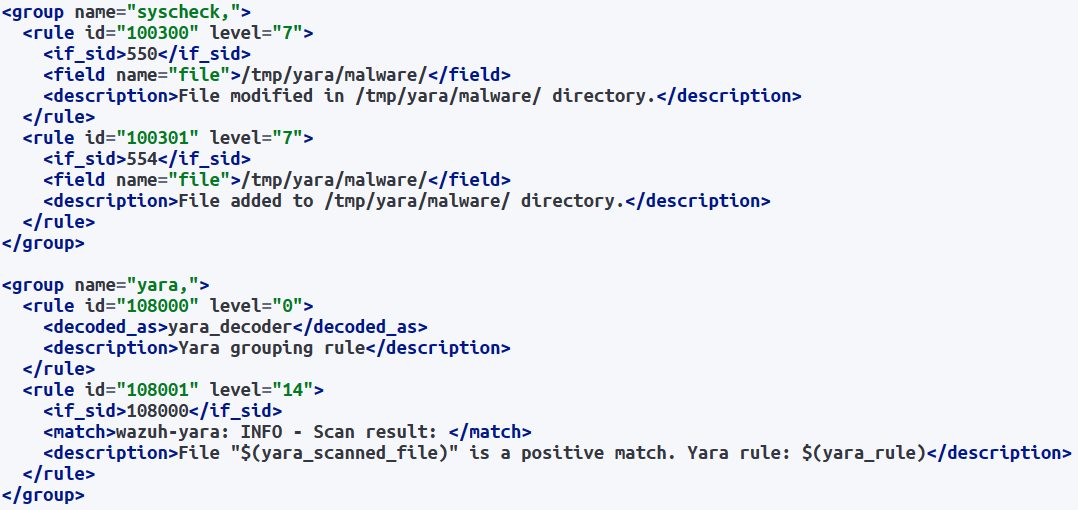
\includegraphics[width=\textwidth]{images/malware-detection/yara/2.png}
        \caption{Custom Rules for YARA Scanning}
        \label{fig:yara-rules}
    \end{figure}

    \item Add the following decoders to the Wazuh server \texttt{/var/ossec/etc/decoders/local/\_decoder.xml} file. This allows extracting the information from YARA scan results.
    \begin{figure}[H]
        \centering
        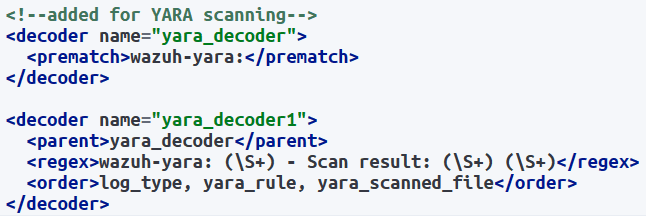
\includegraphics[width=\textwidth]{images/malware-detection/yara/3.png}
        \caption{Custom Decoders for YARA Scanning}
        \label{fig:yara-decoders}
    \end{figure}

    \item Add the following configuration to the Wazuh server \texttt{/var/ossec/etc/ossec.conf} configuration file. This configures the active response module to trigger after the rule 100300 and 100301 are fired.
    \begin{figure}[H]
        \centering
        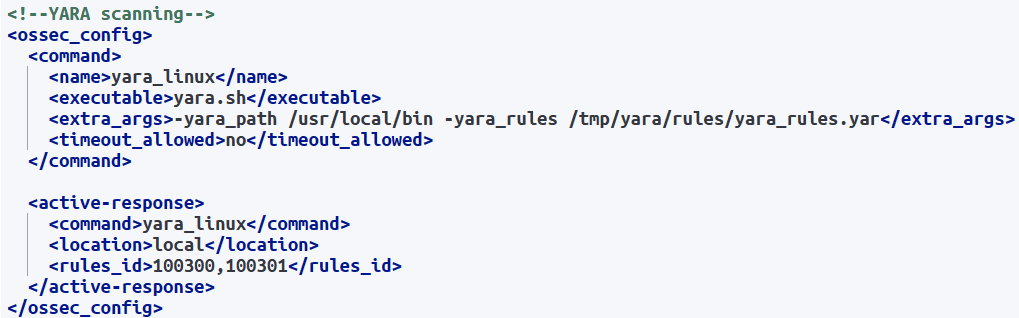
\includegraphics[width=\textwidth]{images/malware-detection/yara/4.png}
        \caption{Updating the Configuration for Active Response}
        \label{fig:yara-config}
    \end{figure}
\end{enumerate}

\paragraph{Simulation}
\begin{enumerate}
    \item Create the script \texttt{/tmp/yara/malware/malware\_downloader.sh} on the monitored endpoint to download malware samples:
    \begin{minted}{bash}
#!/bin/bash
# Wazuh - Malware Downloader for test purposes
# Copyright (C) 2015-2022, Wazuh Inc.
#
# This program is free software; you can redistribute it
# and/or modify it under the terms of the GNU General Public
# License (version 2) as published by the FSF - Free Software
# Foundation.

function fetch_sample(){

  curl -s -XGET "$1" -o "$2"

}

echo "WARNING: Downloading Malware samples, please use this script with  caution."
read -p "  Do you want to continue? (y/n)" -n 1 -r ANSWER
echo

if [[ $ANSWER =~ ^[Yy]$ ]]
then
    echo
    # Mirai
    echo "# Mirai: https://en.wikipedia.org/wiki/Mirai_(malware)"
    echo "Downloading malware sample..."
    fetch_sample "https://wazuh-demo.s3-us-west-1.amazonaws.com/mirai" "/tmp/yara/malware/mirai" && echo "Done!" || echo "Error while downloading."
    echo

    # Xbash
    echo "# Xbash: https://unit42.paloaltonetworks.com/unit42-xbash-combines-botnet-ransomware-coinmining-worm-targets-linux-windows/"
    echo "Downloading malware sample..."
    fetch_sample "https://wazuh-demo.s3-us-west-1.amazonaws.com/xbash" "/tmp/yara/malware/xbash" && echo "Done!" || echo "Error while downloading."
    echo

    # VPNFilter
    echo "# VPNFilter: https://news.sophos.com/en-us/2018/05/24/vpnfilter-botnet-a-sophoslabs-analysis/"
    echo "Downloading malware sample..."
    fetch_sample "https://wazuh-demo.s3-us-west-1.amazonaws.com/vpn_filter" "/tmp/yara/malware/vpn_filter" && echo "Done!" || echo "Error while downloading."
    echo

    # Webshell
    echo "# WebShell: https://github.com/SecWiki/WebShell-2/blob/master/Php/Worse%20Linux%20Shell.php"
    echo "Downloading malware sample..."
    fetch_sample "https://wazuh-demo.s3-us-west-1.amazonaws.com/webshell" "/tmp/yara/malware/webshell" && echo "Done!" || echo "Error while downloading."
    echo
fi
    \end{minted}
    \item Run the \texttt{malware\_downloader.sh} script to download malware samples to the \texttt{/tmp/yara/malware} directory:
    \begin{minted}{bash}
sudo bash /tmp/yara/malware/malware_downloader.sh
    \end{minted}
    \begin{figure}[H]
        \centering
        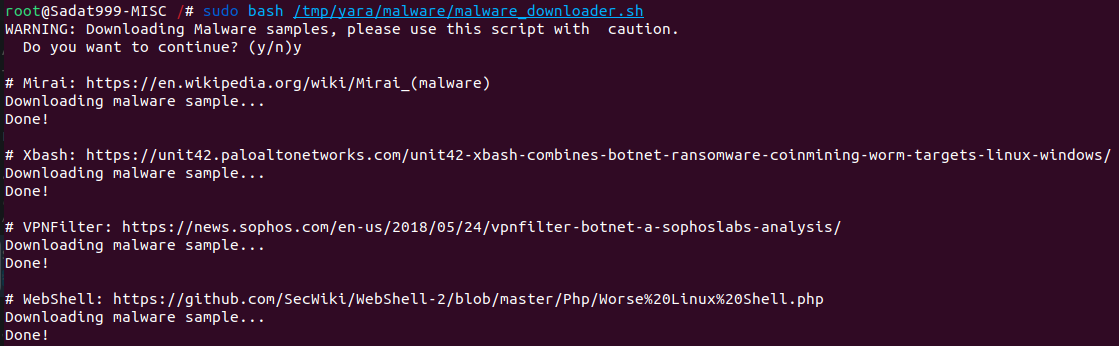
\includegraphics[width=0.75\textwidth]{images/malware-detection/yara/5.png}
        \caption{Downloading Four Malwares for YARA Scanning Simulation}
        \label{fig:yara-malware-download}
    \end{figure}
\end{enumerate}

\paragraph{Dashboard Update}
If we navigate like previously shown in \ref{navigate-sec}, we will see some changes. Number of level 12 or above alerts will go up by quite a bit, because of multiple alert generation for the same malwares. To be precise, they rose by 19. 
    \begin{figure}[H]
        \centering
        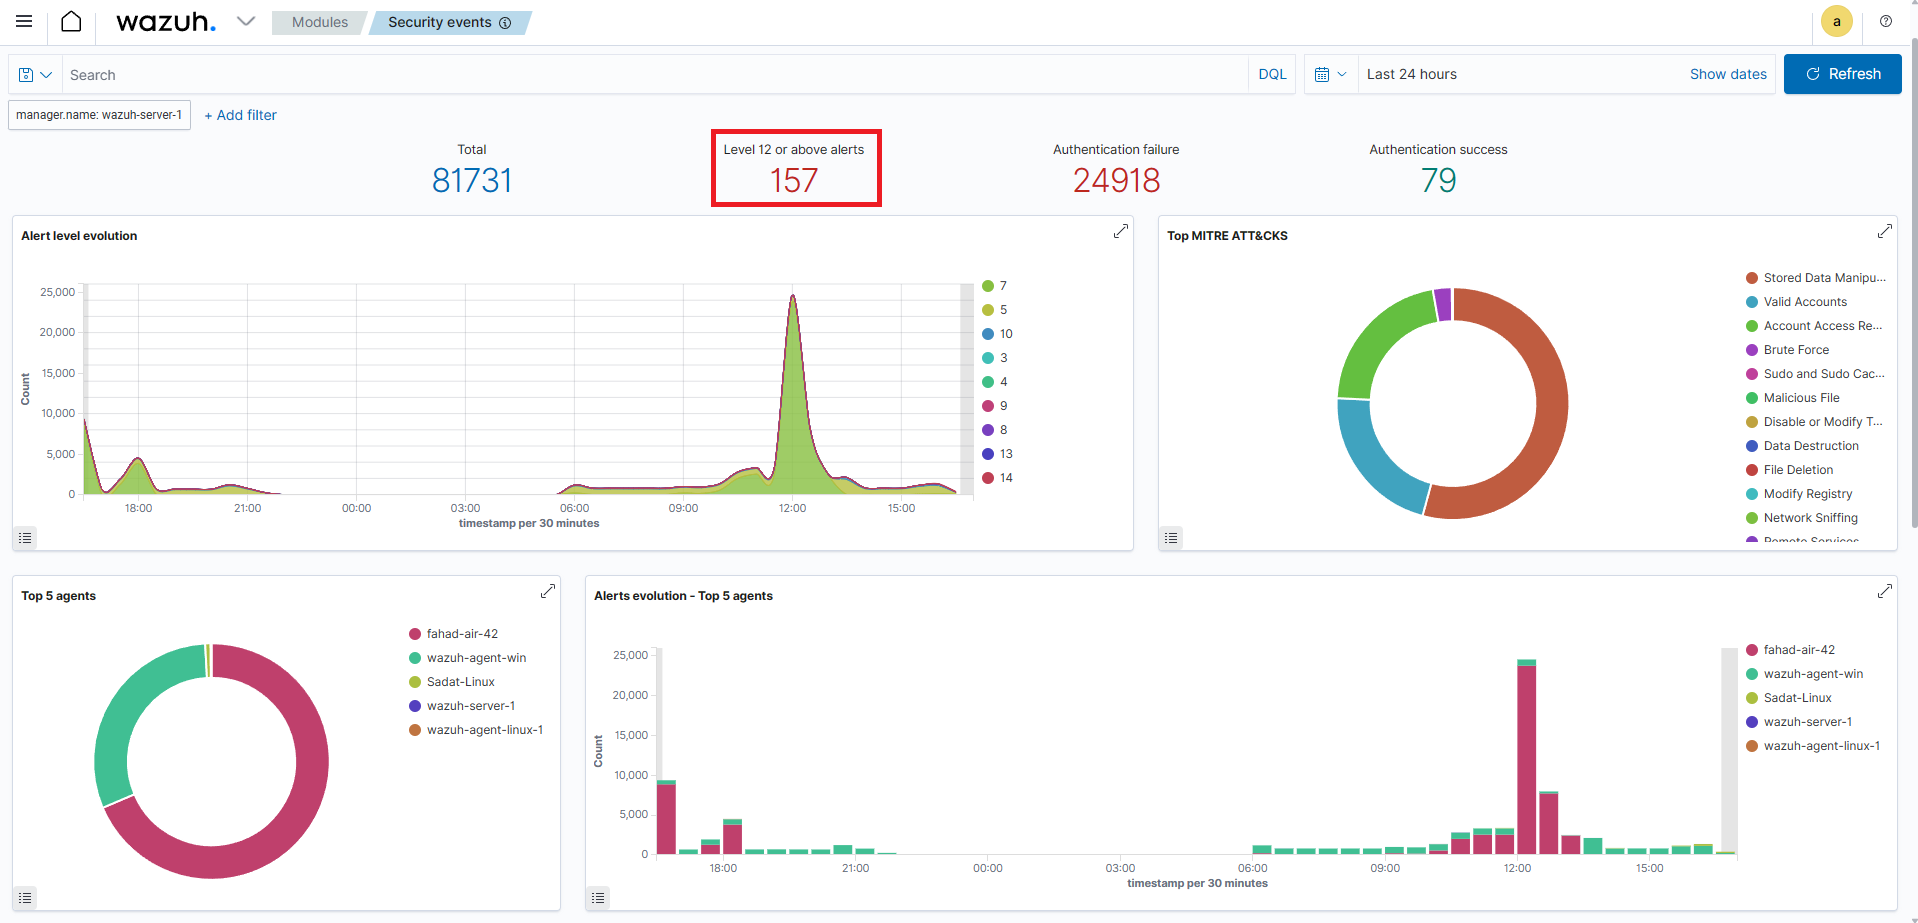
\includegraphics[width=\textwidth]{images/malware-detection/yara/6.png}
        \caption{Dashboard after Downloading the Malwares}
        \label{fig:yara-post-download}
    \end{figure}
If we go to the Events tab, we can see the alerts better. To precisely filter out the alerts generated by YARA, we select,
\begin{minted}{text}
rule.groups:yara
\end{minted}
Then we can see all the generated alerts. Point to be noted here, Wazuh was able to detect all four of the malwares - Mirai, Xbash, VPNFilter and Webshell.
    \begin{figure}[H]
        \centering
        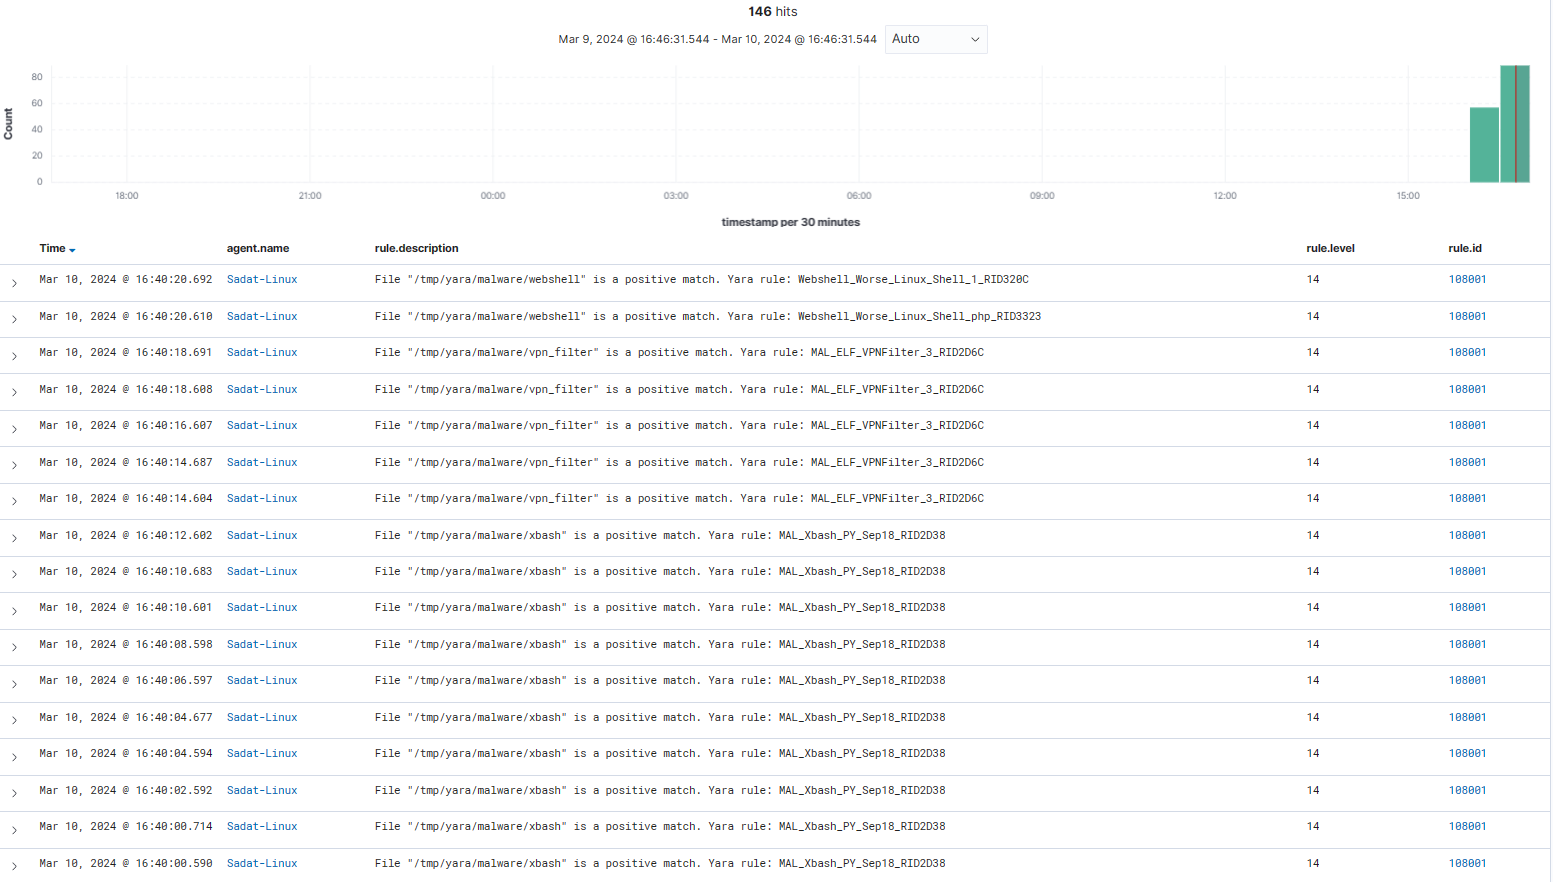
\includegraphics[width=0.55\textwidth]{images/malware-detection/yara/7.png}
        \caption{Generated Alerts after Downloading Four Malwares}
        \label{fig:yara-alerts}
    \end{figure}

\subsubsection{VirusTotal Integration}
\label{virustotal}
VirusTotal is an online service that analyzes files and URLs to detect viruses, worms, trojans, and other malicious content using antivirus engines and website scanners. Since VirusTotal stores all the analyses it performs, users can search for file hashes. VirusTotal also provides an API that allows access to the information generated by VirusTotal without needing to utilize the HTML website interface.

\paragraph{How it works}
This integration leverages the VirusTotal API to identify malicious content in files and directories monitored by the File Integrity Monitoring (FIM) feature of Wazuh. The workflow is outlined as follows:

\begin{enumerate}
    \item The FIM module in Wazuh monitors for any additions, changes, or deletions in the monitored directories, generating alerts for any detected modifications.
    \item Upon detecting a modification, and if the VirusTotal integration is enabled, Wazuh triggers this integration based on the FIM alert. This involves extracting the file's hash and initiating a VirusTotal scan.
    \item The integration executes an HTTP POST request to the VirusTotal database via the VirusTotal API, submitting the file hash for comparison against the VirusTotal database records.
    \item Upon receiving a JSON response from VirusTotal, the integration triggers one of the following types of Wazuh alerts based on the response content:
    \begin{itemize}
        \item \textbf{Error: Check credentials}
        \begin{minted}{json}
{
   "timestamp":"2022-11-17T19:17:43.637+0200",
   "rule":{
      "level":3,
      "description":"VirusTotal: Error: Check credentials",
      "id":"87102",
      "firedtimes":3,
      "mail":false,
      "groups":[
         "virustotal"
      ],
      "gdpr":[
         "IV_35.7.d",
         "IV_32.2"
      ]
   },
   "agent":{
      "id":"000",
      "name":"localhost.localdomain"
   },
   "manager":{
      "name":"localhost.localdomain"
   },
   "id":"1668705463.51155",
   "decoder":{
      "name":"json"
   },
   "data":{
      "virustotal":{
         "error":"403",
         "description":"Error: Check credentials"
      },
      "integration":"virustotal"
   },
   "location":"virustotal"
}
        \end{minted}
        \item \textbf{Error: Public API request rate limit reached}
\begin{minted}{json}
{
   "timestamp":"2022-11-17T19:22:13.236+0200",
   "rule":{
      "level":3,
      "description":"VirusTotal: Error: Public API request rate limit reached",
      "id":"87101",
      "firedtimes":2,
      "mail":false,
      "groups":[
         "virustotal"
      ]
   },
   "agent":{
      "id":"000",
      "name":"localhost.localdomain"
   },
   "manager":{
      "name":"localhost.localdomain"
   },
   "id":"1668705733.90632",
   "decoder":{
      "name":"json"
   },
   "data":{
      "virustotal":{
         "error":"204",
         "description":"Error: Public API request rate limit reached"
      },
      "integration":"virustotal"
   },
   "location":"virustotal"
}
\end{minted}
        \item \textbf{Alert: No positives found}
\begin{minted}{json}
{
   "timestamp":"2022-11-17T19:22:07.974+0200",
   "rule":{
      "level":3,
      "description":"VirusTotal: Alert - /media/user/software/suspicious-file10.exe \
      - No positives found",
      "id":"87104",
      "firedtimes":4,
      "mail":false,
      "groups":[
         "virustotal"
      ]
   },
   "agent":{
      "id":"010",
      "name":"Ubuntu",
      "ip":"10.0.2.15"
   },
   "manager":{
      "name":"localhost.localdomain"
   },
   "id":"1668705727.84464",
   "decoder":{
      "name":"json"
   },
   "data":{
      "virustotal":{
         "found":"1",
         "malicious":"0",
         "source":{
            "alert_id":"1668705721.82254",
            "file":"/media/user/software/suspicious-file10.exe",
            "md5":"d41d8cd98f00b204e9800998ecf8427e",
            "sha1":"da39a3ee5e6b4b0d3255bfef95601890afd80709"
         },
         "sha1":"da39a3ee5e6b4b0d3255bfef95601890afd80709",
         "scan_date":"2022-11-17 17:19:48",
         "positives":"0",
         "total":"60",
         "permalink":"https://www.virustotal.com/gui/file/e3b0c44298fc1c149afbf\
         4c8996fb92427ae41e4649b934ca495991b7852b855/detection/f-e3b0c44298fc1c\
         149afbf4c8996fb92427ae41e4649b934ca495991b7852b855-1668705588"
      },
      "integration":"virustotal"
   },
   "location":"virustotal"
}
\end{minted}
        \item \textbf{Alert: X engines detected this file}
        Here, X represents the number of antivirus engines that flagged the file.
    \begin{minted}{json}
{
   "timestamp":"2022-11-17T19:30:25.085+0200",
   "rule":{
      "level":12,
      "description":"VirusTotal: Alert - /media/user/software/eicar.com - 66 engines detected this file",
      "id":"87105",
      "mitre":{
         "id":[
            "T1203"
         ],
         "tactic":[
            "Execution"
         ],
         "technique":[
            "Exploitation for Client Execution"
         ]
      },
      "firedtimes":1,
      "mail":true,
      "groups":[
         "virustotal"
      ],
      "pci_dss":[
         "10.6.1",
         "11.4"
      ],
      "gdpr":[
         "IV_35.7.d"
      ]
   },
   "agent":{
      "id":"010",
      "name":"Ubuntu",
      "ip":"10.0.2.15"
   },
   "manager":{
      "name":"localhost.localdomain"
   },
   "id":"1668706225.104492",
   "decoder":{
      "name":"json"
   },
   "data":{
      "virustotal":{
         "found":"1",
         "malicious":"1",
         "source":{
            "alert_id":"1668706222.103798",
            "file":"/media/user/software/eicar.com",
            "md5":"44d88612fea8a8f36de82e1278abb02f",
            "sha1":"3395856ce81f2b7382dee72602f798b642f14140"
         },
         "sha1":"3395856ce81f2b7382dee72602f798b642f14140",
         "scan_date":"2022-11-17 17:15:04",
         "positives":"66",
         "total":"68",
         "permalink":"https://www.virustotal.com/gui/file/275a021bb\
         fb6489e54d471899f7db9d1663fc695ec2fe2a2c4538aabf651fd0f\
         /detection/f-275a021bbfb6489e54d471899f7db9d1663fc695ec2fe2a2c4538aabf651fd0f-1668705304"
      },
      "integration":"virustotal"
   },
   "location":"virustotal"
}
    \end{minted}
    \end{itemize}
\end{enumerate}

\paragraph{Configuration}
\subparagraph{Linux endpoint}
\begin{enumerate}
    \item Add the following to the \texttt{\textlangle syscheck\textrangle} section of the configuration file. We reuse the same folder \texttt{/fim} as previously used in \ref{fim-source}. If that configuration is already done, the following no more needs to be added.
    \begin{minted}{xml}
<syscheck>
  <directories check_all="yes" realtime="yes">/fim</directories>
</syscheck>
    \end{minted}

    \item Restart the Wazuh manager.
    \begin{minted}{bash}
systemctl restart wazuh-manager
    \end{minted}
\end{enumerate}

\subparagraph{Wazuh server}
\begin{enumerate}
    \item Add the following to the \texttt{/var/ossec/etc/ossec.conf} file on the Wazuh server:
    \begin{figure}[H]
        \centering
        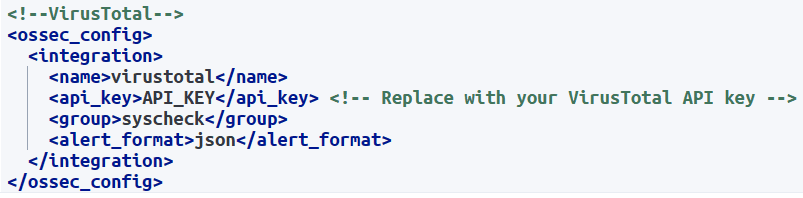
\includegraphics[width=\textwidth]{images/malware-detection/virustotal/1.png}
        \caption{Configuration for VirusTotal Integration}
        \label{fig:virustotal-conf}
    \end{figure}
\end{enumerate}

\paragraph{Simulation}
\begin{enumerate}
    \item Download a malicious file on the endpoint in the monitored folder.
    \begin{minted}{bash}
sudo curl -Lo /fim/suspicious-file.exe https://secure.eicar.org/eicar.com
    \end{minted}
    \begin{figure}[H]
        \centering
        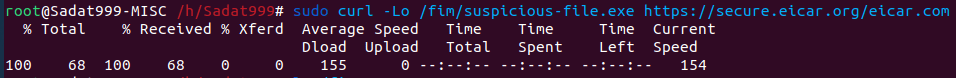
\includegraphics[width=\textwidth]{images/malware-detection/virustotal/2.png}
        \caption{Downloading Malware for VirusTotal Checking}
        \label{fig:virustotal-malware}
    \end{figure}
\end{enumerate}

\paragraph{Dashboard Update}
We will again navigate to ``Security events" tab as shown previously in \ref{navigate-sec}. There we will see a new level 12 alert has been generated because of the malware download (the count was previously 179).
    \begin{figure}[H]
        \centering
        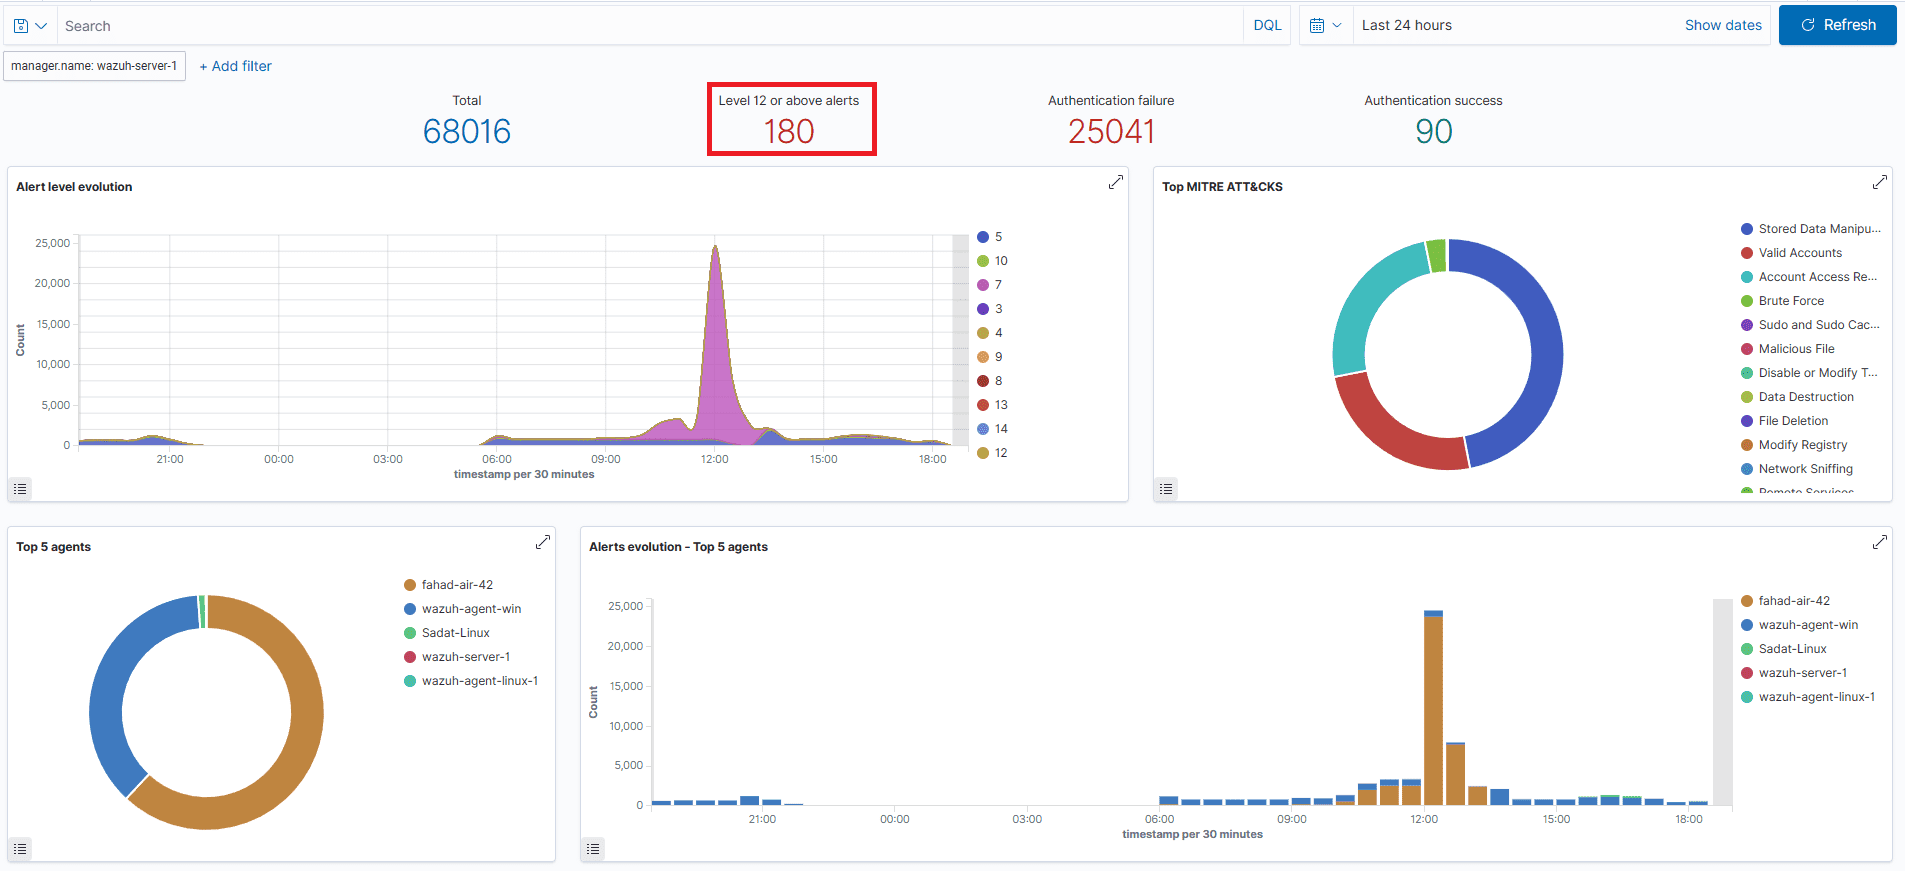
\includegraphics[width=\textwidth]{images/malware-detection/virustotal/3.png}
        \caption{Dashboard after Malware Download}
        \label{fig:virustotal-post-download}
    \end{figure}
The generated alert goes as follows:
    \begin{figure}[H]
        \centering
        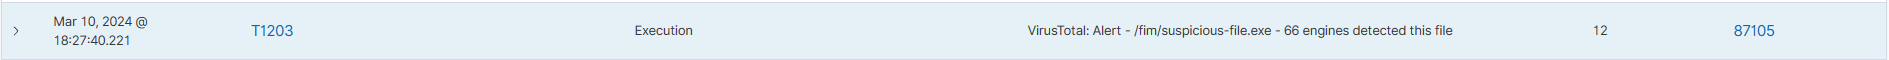
\includegraphics[width=\textwidth]{images/malware-detection/virustotal/4.png}
        \caption{Alert Generated by VirusTotal API Check}
        \label{fig:virustotal-alert}
    \end{figure}
If we examine the JSON body of the alert, we can see that 66 engines or anti-virus softwares, out of 68, flagged our downloaded file as a malware.
\begin{minted}{json}
{
  "agent": {
    "ip": "10.0.0.4",
    "name": "Sadat-Linux",
    "id": "008"
  },
  "manager": {
    "name": "wazuh-server-1"
  },
  "data": {
    "integration": "virustotal",
    "virustotal": {
      "sha1": "3395856ce81f2b7382dee72602f798b642f14140",
      "malicious": "1",
      "total": "68",
      "found": "1",
      "positives": "66",
      "source": {
        "sha1": "3395856ce81f2b7382dee72602f798b642f14140",
        "file": "/fim/suspicious-file.exe",
        "alert_id": "1710073657.200258194",
        "md5": "44d88612fea8a8f36de82e1278abb02f"
      },
      "permalink": "https://www.virustotal.com/gui/file/275a021bbfb6489e54d471899f7db9d1663fc695ec2fe2a2c4538aabf651fd0f/detection/f-275a021bbfb6489e54d471899f7db9d1663fc695ec2fe2a2c4538aabf651fd0f-1710073285",
      "scan_date": "2024-03-10 12:21:25"
    }
  },
  "rule": {
    "firedtimes": 1,
    "mail": true,
    "level": 12,
    "pci_dss": [
      "10.6.1",
      "11.4"
    ],
    "description": "VirusTotal: Alert - /fim/suspicious-file.exe - 66 engines detected this file",
    "groups": [
      "virustotal"
    ],
    "mitre": {
      "technique": [
        "Exploitation for Client Execution"
      ],
      "id": [
        "T1203"
      ],
      "tactic": [
        "Execution"
      ]
    },
    "id": "87105",
    "gdpr": [
      "IV_35.7.d"
    ]
  },
  "decoder": {
    "name": "json"
  },
  "input": {
    "type": "log"
  },
  "@timestamp": "2024-03-10T12:27:40.221Z",
  "location": "virustotal",
  "id": "1710073660.200290701",
  "timestamp": "2024-03-10T12:27:40.221+0000",
  "_id": "6JBVKI4B8KVEhOwaUUG9"
}
\end{minted}

\subsubsection{Windows Defender Logs Collection}
Windows Defender is the anti-malware component of the Microsoft Windows operating system. Wazuh agents installed on Windows endpoints can be configured to collect Windows Defender logs. This provides visibility on malware infections detected by Windows Defender on Windows endpoints. These logs can provide information about:
\begin{itemize}
    \item The status of the Windows Defender service.
    \item Results of Windows Defender scans that the users run on these endpoints.
\end{itemize}

\paragraph{How it works}
Wazuh has out-of-the-box decoders for Microsoft Windows logs including Windows Defender. Rules are also included specifically for Windows Defender, which can be found at \texttt{/var/ossec/ruleset/rules/0600-win-wdefender\_rules.xml} on the Wazuh server. Below are examples of Windows Defender alerts, which are triggered by user and malware activity.

\begin{itemize}
    \item \textbf{Windows Defender detects malware}
    \hypertarget{detect-malware}{}
    \begin{minted}{json}
{
   "timestamp":"2023-01-05T11:44:58.557+0200",
   "rule":{
      "level":12,
      "description":"Windows Defender: Antimalware platform detected  potentially unwanted software ()",
      "id":"62123",
      "firedtimes":2,
      "mail":true,
      "groups":[
         "windows",
         "windows_defender"
      ],
      "pci_dss":[
         "5.1",
         "5.2",
         "10.6.1",
         "11.4"
      ],
      "gpg13":[
         "4.2"
      ],
      "gdpr":[
         "IV_35.7.d"
      ],
      "hipaa":[
         "164.312.b"
      ],
      "nist_800_53":[
         "SI.3",
         "AU.6",
         "SI.4"
      ],
      "tsc":[
         "A1.2",
         "CC7.2",
         "CC7.3",
         "CC6.1",
         "CC6.8"
      ]
   },
   "agent":{
      "id":"012",
      "name":"Windows_11",
      "ip":"10.0.2.15"
   },
   "manager":{
      "name":"localhost.localdomain"
   },
   "id":"1672911898.1113167",
   "decoder":{
      "name":"windows_eventchannel"
   },
   "data":{
      "win":{
         "system":{
            "providerName":"Microsoft-Windows-Windows Defender",
            "providerGuid":"{11cd958a-c507-4ef3-b3f2-5fd9dfbd2c78}",
            "eventID":"1116",
            "version":"0",
            "level":"3",
            "task":"0",
            "opcode":"0",
            "keywords":"0x8000000000000000",
            "systemTime":"2023-01-05T09:44:55.1124563Z",
            "eventRecordID":"525",
            "processID":"2600",
            "threadID":"432",
            "channel":"Microsoft-Windows-Windows Defender/Operational",
            "computer":"Windows-11",
            "severityValue":"WARNING",
            "message":"\"Microsoft Defender Antivirus has detected malware or other potentially unwanted software.\r\n For more information please see the following:\r\nhttps://go.microsoft.com/fwlink/?linkid=37020&name=Virus:DOS/EICAR_Test_File&threatid=2147519003&enterprise=0\r\n \tName: Virus:DOS/EICAR_Test_File\r\n \tID: 2147519003\r\n \tSeverity: Severe\r\n \tCategory: Virus\r\n \tPath: file:_C:\\Users\\win11\\AppData\\Local\\Temp\\36f9c971-77e5-4f5e-bbef-f7162522dee1.tmp; webfile:_C:\\Users\\win11\\AppData\\Local\\Temp\\36f9c971-77e5-4f5e-bbef-f7162522dee1.tmp|https://secure.eicar.org/eicar.com.txt|pid:8412,ProcessStart:133173854939240064\r\n \tDetection Origin: Internet\r\n \tDetection Type: Concrete\r\n \tDetection Source: Downloads and attachments\r\n \tUser: Windows-11\\win11\r\n \tProcess Name: Unknown\r\n \tSecurity intelligence Version: AV: 1.381.1755.0, \
            AS: 1.381.1755.0, NIS: 1.381.1755.0\r\n \tEngine Version: AM: 1.1.19900.2, NIS: 1.1.19900.2\""
         },
         "eventdata":{
            "product Name":"Microsoft Defender Antivirus",
            "product Version":"4.18.2211.5",
            "detection ID":"{53737EEC-A8A6-45E0-9155-4566B8133573}",
            "detection Time":"2023-01-05T09:44:55.064Z",
            "threat ID":"2147519003",
            "threat Name":"Virus:DOS/EICAR_Test_File",
            "severity ID":"5",
            "severity Name":"Severe",
            "category ID":"42",
            "category Name":"Virus",
            "fWLink":"https://go.microsoft.com/fwlink/?linkid=37020&amp;name=Virus:DOS/EICAR_Test_File&amp;threatid=2147519003&amp;enterprise=0",
            "status Code":"1",
            "state":"1",
            "source ID":"4",
            "source Name":"Downloads and attachments",
            "process Name":"Unknown",
            "detection User":"Windows-11\\\\win11",
            "path":"file:_C:\\\\Users\\\\win11\\\\AppData\\\\Local\\\\Temp\\\\36f9c971-77e5-4f5e-bbef-f7162522dee1.tmp; webfile:_C:\\\\Users\\\\win11\\\\AppData\\\\Local\\\\Temp\\\\36f9c971-77e5-4f5e-bbef-f7162522dee1.tmp|https://secure.eicar.org/eicar.com.txt|pid:8412,ProcessStart:133173854939240064",
            "origin ID":"4",
            "origin Name":"Internet",
            "execution ID":"0",
            "execution Name":"Unknown",
            "type ID":"0",
            "type Name":"Concrete",
            "pre Execution Status":"0",
            "action ID":"9",
            "action Name":"Not Applicable",
            "error Code":"0x00000000",
            "error Description":"The operation completed successfully.",
            "post Clean Status":"0",
            "additional Actions ID":"0",
            "additional Actions String":"No additional actions required",
            "security intelligence Version":"AV: 1.381.1755.0, AS: 1.381.1755.0, NIS: 1.381.1755.0",
            "engine Version":"AM: 1.1.19900.2, NIS: 1.1.19900.2"
         }
      }
   },
   "location":"EventChannel"
}
    \end{minted}

    \item \textbf{Windows Defender responds to detected malware}
    \hypertarget{response-malware}{}
    \begin{minted}{json}
{
   "timestamp":"2023-01-05T11:45:06.032+0200",
   "rule":{
      "level":3,
      "description":"Windows Defender: Antimalware platform performed an action to protect you from potentially unwanted software ()",
      "id":"62124",
      "firedtimes":2,
      "mail":false,
      "groups":[
         "windows",
         "windows_defender"
      ],
      "pci_dss":[
         "5.1",
         "5.2",
         "10.6.1",
         "11.4"
      ],
      "gpg13":[
         "4.2"
      ],
      "gdpr":[
         "IV_35.7.d"
      ],
      "hipaa":[
         "164.312.b"
      ],
      "nist_800_53":[
         "SI.3",
         "AU.6",
         "SI.4"
      ],
      "tsc":[
         "A1.2",
         "CC7.2",
         "CC7.3",
         "CC6.1",
         "CC6.8"
      ]
   },
   "agent":{
      "id":"012",
      "name":"Windows_11",
      "ip":"10.0.2.15"
   },
   "manager":{
      "name":"localhost.localdomain"
   },
   "id":"1672911906.1119694",
   "decoder":{
      "name":"windows_eventchannel"
   },
   "data":{
      "win":{
         "system":{
            "providerName":"Microsoft-Windows-Windows Defender",
            "providerGuid":"{11cd958a-c507-4ef3-b3f2-5fd9dfbd2c78}",
            "eventID":"1117",
            "version":"0",
            "level":"4",
            "task":"0",
            "opcode":"0",
            "keywords":"0x8000000000000000",
            "systemTime":"2023-01-05T09:45:02.6103899Z",
            "eventRecordID":"526",
            "processID":"2600",
            "threadID":"432",
            "channel":"Microsoft-Windows-Windows Defender/Operational",
            "computer":"Windows-11",
            "severityValue":"INFORMATION",
            "message": "Microsoft Defender Antivirus has taken action to protect this machine from malware or other potentially unwanted software. \
            For more information please see the following: \
            https://go.microsoft.com/fwlink/?linkid=37020&name=Virus:DOS/EICAR_Test_File&threatid=2147519003&enterprise=0 \
            \tName: Virus:DOS/EICAR_Test_File \
            \tID: 2147519003 \
            \tSeverity: Severe \
            \tCategory: Virus \
            \tPath: file:_C:\\Users\\win11\\AppData\\Local\\Temp\\36f9c971-77e5-4f5e-bbef-f7162522dee1.tmp; webfile:_C:\\Users\\win11\\AppData\\Local\\Temp\\36f9c971-77e5-4f5e-bbef-f7162522dee1.tmp|https://secure.eicar.org/eicar.com.txt|pid:8412,ProcessStart:133173854939240064 \
            \tDetection Origin: Internet \
            \tDetection Type: Concrete \
            \tDetection Source: Downloads and attachments \
            \tUser: NT AUTHORITY\\SYSTEM \
            \tProcess Name: Unknown \
            \tAction: Quarantine \
            \tAction Status: No additional actions required \
            \tError Code: 0x00000000 \
            \tError description: The operation completed successfully. \
            \tSecurity intelligence Version: AV: 1.381.1755.0, AS: 1.381.1755.0, NIS: 1.381.1755.0 \
            \tEngine Version: AM: 1.1.19900.2, NIS: 1.1.19900.2"
         },
         "eventdata":{
            "product Name":"Microsoft Defender Antivirus",
            "product Version":"4.18.2211.5",
            "detection ID":"{53737EEC-A8A6-45E0-9155-4566B8133573}",
            "detection Time":"2023-01-05T09:44:55.064Z",
            "threat ID":"2147519003",
            "threat Name":"Virus:DOS/EICAR_Test_File",
            "severity ID":"5",
            "severity Name":"Severe",
            "category ID":"42",
            "category Name":"Virus",
            "fWLink":"https://go.microsoft.com/fwlink/?linkid=37020&amp;name=Virus:DOS/EICAR_Test_File&amp;threatid=2147519003&amp;enterprise=0",
            "status Code":"4",
            "state":"2",
            "source ID":"4",
            "source Name":"Downloads and attachments",
            "process Name":"Unknown",
            "detection User":"Windows-11\\\\win11",
            "path":"file:_C:\\\\Users\\\\win11\\\\AppData\\\\Local\\\\Temp\\\\36f9c971-77e5-4f5e-bbef-f7162522dee1.tmp; webfile:_C:\\\\Users\\\\win11\\\\AppData\\\\Local\\\\Temp\\\\36f9c971-77e5-4f5e-bbef-f7162522dee1.tmp|https://secure.eicar.org/eicar.com.txt|pid:8412,ProcessStart:133173854939240064",
            "origin ID":"4",
            "origin Name":"Internet",
            "execution ID":"0",
            "execution Name":"Unknown",
            "type ID":"0",
            "type Name":"Concrete",
            "pre Execution Status":"0",
            "action ID":"2",
            "action Name":"Quarantine",
            "error Code":"0x00000000",
            "error Description":"The operation completed successfully.",
            "post Clean Status":"0",
            "additional Actions ID":"0",
            "additional Actions String":"No additional actions required",
            "remediation User":"NT AUTHORITY\\\\SYSTEM",
            "security intelligence Version":"AV: 1.381.1755.0, AS: 1.381.1755.0, NIS: 1.381.1755.0",
            "engine Version":"AM: 1.1.19900.2, NIS: 1.1.19900.2"
         }
      }
   },
   "location":"EventChannel"
}
    \end{minted}

    \item \textbf{Windows Defender protection is disabled}
    \hypertarget{defender-disabled}{}
    \begin{minted}{json}
{
   "timestamp":"2023-01-05T16:26:55.513+0200",
   "rule":{
      "level":5,
      "description":"Windows Defender: Antivirus real-time protection is disabled",
      "id":"62152",
      "firedtimes":1,
      "mail":false,
      "groups":[
         "windows",
         "windows_defender"
      ],
      "pci_dss":[
         "5.1",
         "10.2.6",
         "10.6.1"
      ],
      "gpg13":[
         "4.14",
         "10.1"
      ],
      "gdpr":[
         "IV_35.7.d"
      ],
      "hipaa":[
         "164.312.b"
      ],
      "nist_800_53":[
         "SI.3",
         "AU.14",
         "AU.5",
         "AU.6"
      ],
      "tsc":[
         "A1.2",
         "CC6.8",
         "CC7.2",
         "CC7.3"
      ]
   },
   "agent":{
      "id":"012",
      "name":"Windows_11",
      "ip":"10.0.2.15"
   },
   "manager":{
      "name":"localhost.localdomain"
   },
   "id":"1672928815.1914866",
   "decoder":{
      "name":"windows_eventchannel"
   },
   "data":{
      "win":{
         "system":{
            "providerName":"Microsoft-Windows-Windows Defender",
            "providerGuid":"{11cd958a-c507-4ef3-b3f2-5fd9dfbd2c78}",
            "eventID":"5001",
            "version":"0",
            "level":"4",
            "task":"0",
            "opcode":"0",
            "keywords":"0x8000000000000000",
            "systemTime":"2023-01-05T14:33:13.3093446Z",
            "eventRecordID":"540",
            "processID":"2600",
            "threadID":"7152",
            "channel":"Microsoft-Windows-Windows Defender/Operational",
            "computer":"Windows-11",
            "severityValue":"INFORMATION",
            "message":"\"Microsoft Defender Antivirus Real-time Protection scanning for malware and other potentially unwanted software was disabled.\""
         },
         "eventdata":{
            "product Name":"Microsoft Defender Antivirus",
            "product Version":"4.18.2211.5"
         }
      }
   },
   "location":"EventChannel"
}
    \end{minted}

    \item \textbf{Windows Defender updates its signature database}
    \hypertarget{defender-update}{}
    \begin{minted}{json}
{
   "timestamp":"2023-01-05T12:55:10.920+0200",
   "rule":{
      "level":3,
      "description":"Windows Defender: Antimalware definitions updated successfully",
      "id":"62130",
      "firedtimes":2,
      "mail":false,
      "groups":[
         "windows",
         "windows_defender"
      ],
      "pci_dss":[
         "5.1",
         "10.6.1",
         "5.2"
      ],
      "gdpr":[
         "IV_35.7.d",
         "IV_35.7.d"
      ],
      "gpg13":[
         "4.4",
         "4.14"
      ],
      "hipaa":[
         "164.312.b"
      ],
      "nist_800_53":[
         "SI.3",
         "AU.6"
      ],
      "tsc":[
         "A1.2",
         "CC7.2",
         "CC7.3"
      ]
   },
   "agent":{
      "id":"011",
      "name":"ONEBOT-1",
      "ip":"10.5.0.2"
   },
   "manager":{
      "name":"localhost.localdomain"
   },
   "id":"1672916110.1441972",
   "decoder":{
      "name":"windows_eventchannel"
   },
   "data":{
      "win":{
         "system":{
            "providerName":"Microsoft-Windows-Windows Defender",
            "providerGuid":"{11cd958a-c507-4ef3-b3f2-5fd9dfbd2c78}",
            "eventID":"2000",
            "version":"0",
            "level":"4",
            "task":"0",
            "opcode":"0",
            "keywords":"0x8000000000000000",
            "systemTime":"2023-01-05T10:55:07.4095656Z",
            "eventRecordID":"649",
            "processID":"6716",
            "threadID":"7528",
            "channel":"Microsoft-Windows-Windows Defender/Operational",
            "computer":"ONEBOT-1",
            "severityValue":"INFORMATION",
            "message":"\"Microsoft Defender Antivirus security intelligence version updated.\r\n \tCurrent security intelligence Version: 1.381.1755.0\r\n \tPrevious security intelligence Version: 1.381.1746.0\r\n \tSecurity intelligence Type: AntiSpyware\r\n \tUpdate Type: Delta\r\n \tUser: NT AUTHORITY\\SYSTEM\r\n \tCurrent Engine Version: 1.1.19900.2\r\n \tPrevious Engine Version: 1.1.19900.2\""
         },
         "eventdata":{
            "product Name":"Microsoft Defender Antivirus",
            "product Version":"4.18.2211.5",
            "current security intelligence Version":"1.381.1755.0",
            "previous security intelligence Version":"1.381.1746.0",
            "domain":"NT AUTHORITY",
            "user":"SYSTEM",
            "sID":"S-1-5-18",
            "security intelligence Type Index":"2",
            "security intelligence Type":"AntiSpyware",
            "update Type Index":"2",
            "update Type":"Delta",
            "current Engine Version":"1.1.19900.2",
            "previous Engine Version":"1.1.19900.2"
         }
      }
   },
   "location":"EventChannel"
}
    \end{minted}
\end{itemize}

\paragraph{Configuration}
\begin{enumerate}
    \item To collect Windows Defender logs, either the centralized configuration can be updated, or locally the agent \texttt{C:\textbackslash Program Files (x86)\textbackslash ossec-agent\textbackslash ossec.conf} file. Centralized configuration allows the instructions to be shared with a group of agents.
    We first navigate to the local configuration file.
    \begin{figure}[H]
        \centering
        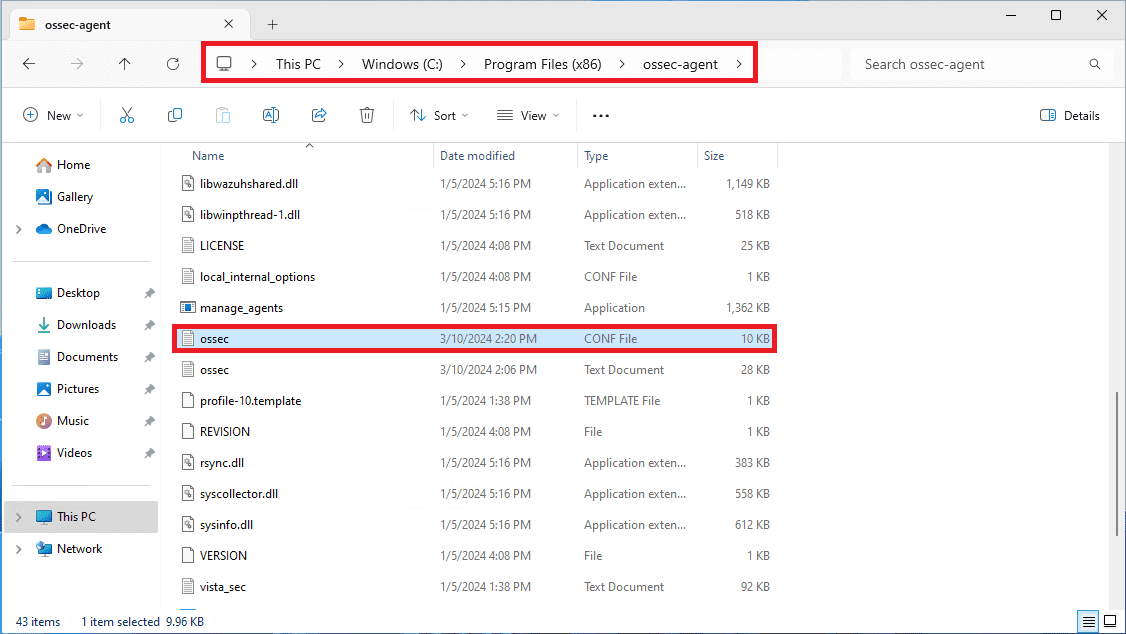
\includegraphics[width=\textwidth]{images/malware-detection/windows-log/1.png}
        \caption{Navigation for Windows Local Configuration File}
        \label{fig:win-conf-navigate}
    \end{figure}
    We then add the following block to the \texttt{ossec.conf} file.
    \begin{minted}{xml}
<localfile>
  <location>Microsoft-Windows-Windows Defender/Operational</location>
  <log_format>eventchannel</log_format>
</localfile>
    \end{minted}

    \item As always, we need to restart the Wazuh agent.
    \begin{minted}{powershell}
NET STOP WazuhSvc
NET START WazuhSvc
    \end{minted}
\end{enumerate}

\paragraph{Simulation}
\begin{enumerate}
    \item We first run a quick scan to assign Windows Defender some work.
    \begin{figure}[H]
        \centering
        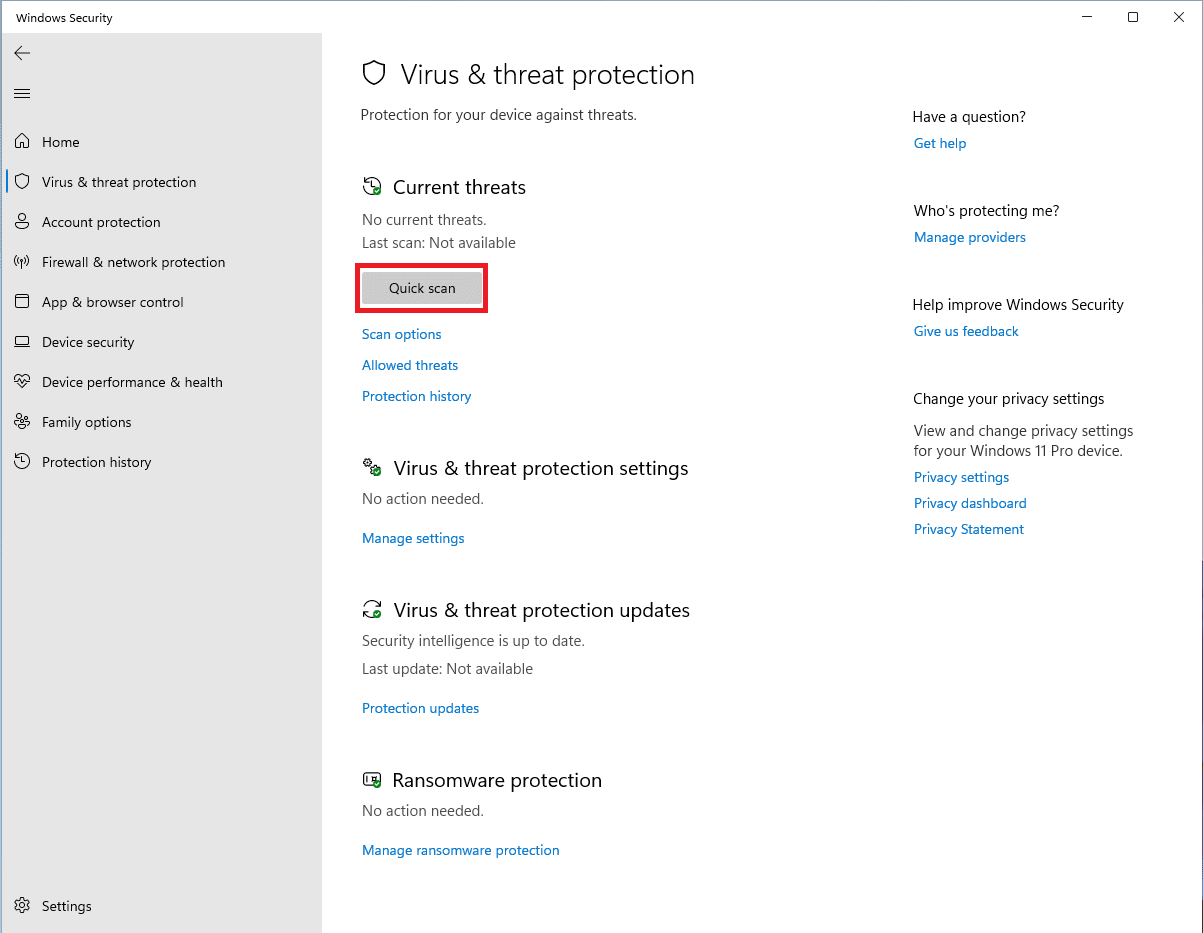
\includegraphics[width=\textwidth]{images/malware-detection/windows-log/2.png}
        \caption{Initiating a Quick Scan on Windows Defender}
        \label{fig:win-quick-scan}
    \end{figure}
    \item After the scan finished, we disable the Real-time protection to trigger an alert.
    \begin{figure}[H]
        \centering
        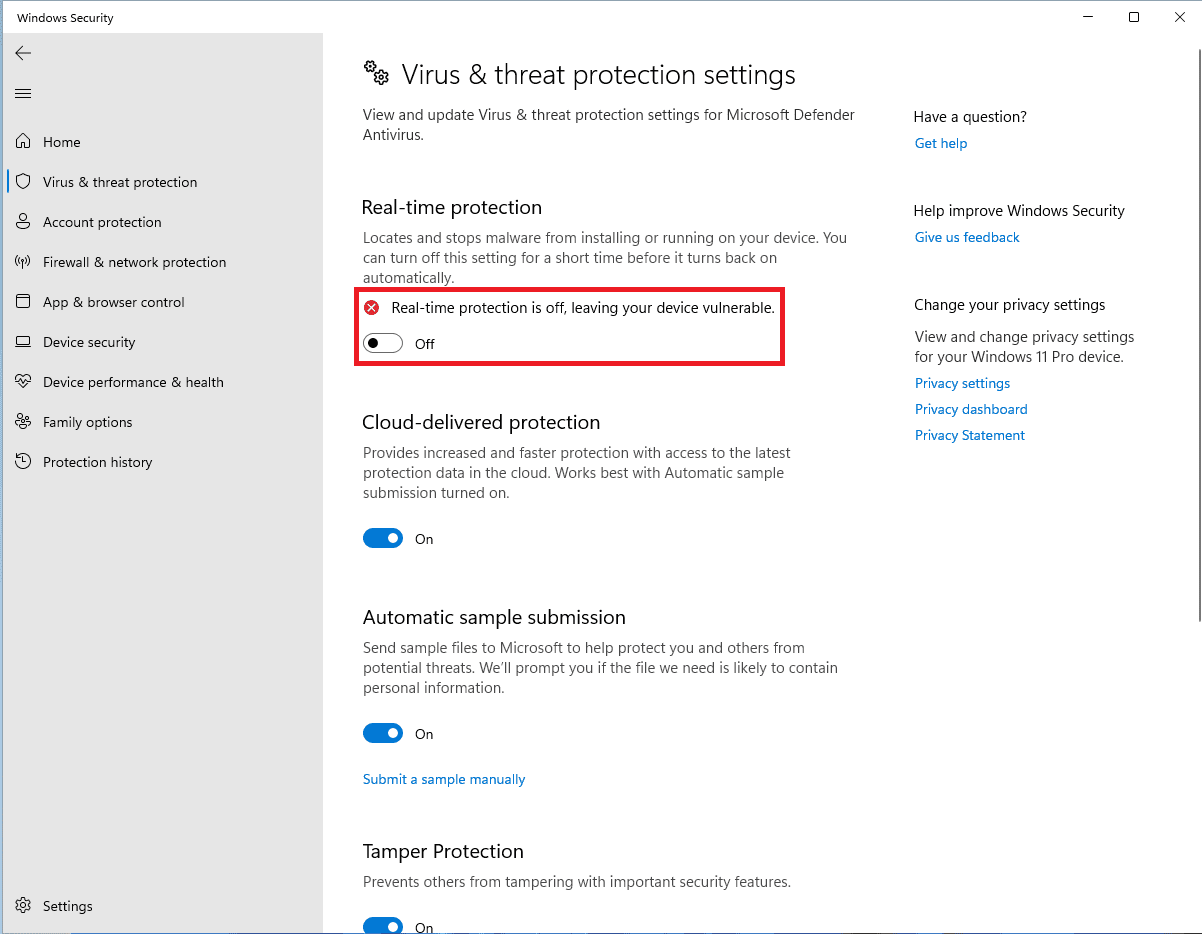
\includegraphics[width=0.5\textwidth]{images/malware-detection/windows-log/3.png}
        \caption{Disabling Realtime Protection}
        \label{fig:win-disable-defender}
    \end{figure}
    \item Lastly, we turn the defender back on and run the following command to download the malware ``eicar".
    \begin{minted}{powershell}
Invoke-WebRequest -Uri https://secure.eicar.org/eicar_com.zip -OutFile eicar.zip
    \end{minted}
    Expectedly, it gets instantly deleted by Windows Defender, but we are more curious to see if it shows up on Wazuh dashboard.
\end{enumerate}

\paragraph{Dashboard Update}
Number of level 12 or above alerts go up by 2 because of the malware download.
    \begin{figure}[H]
        \centering
        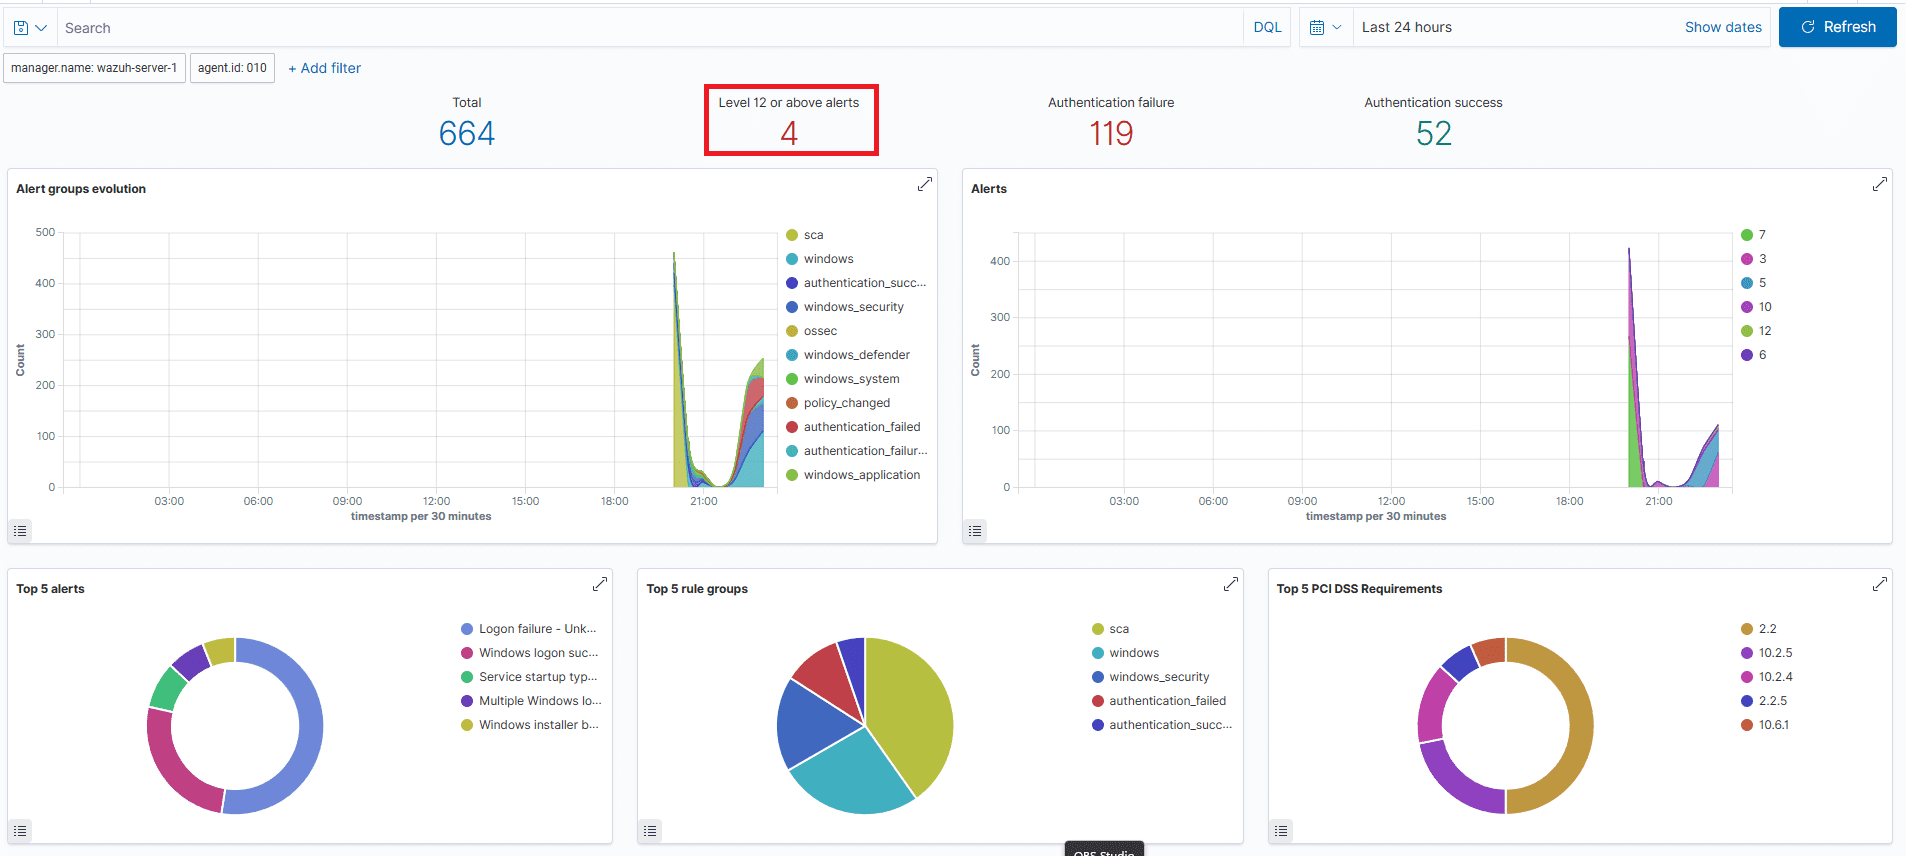
\includegraphics[width=\textwidth]{images/malware-detection/windows-log/5.png}
        \caption{Dashboard after Security Events on Windows Client}
        \label{fig:win-dashboard}
    \end{figure}
We can also see all the alerts generated because of our triggering events. The alerts are generated, as previously described in \hyperlink{defender-disabled}{Defender Disabled}, \hyperlink{detect-malware}{Malware Detected} and \hyperlink{response-malware}{Malware Response}.
    \begin{figure}[H]
        \centering
        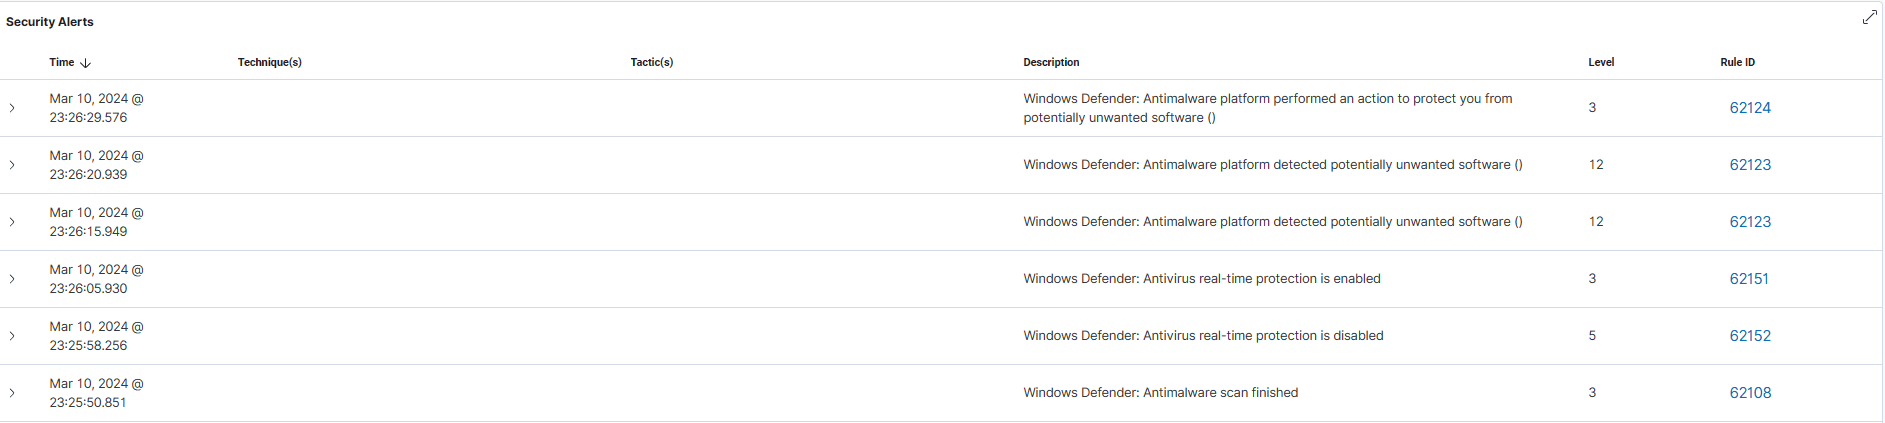
\includegraphics[width=\textwidth]{images/malware-detection/windows-log/4.png}
        \caption{Generated Alerts from Windows Defender}
        \label{fig:win-def-alerts}
    \end{figure}
